\subsection{Detección de marcadores}
El bloque de detección de marcadores, se puede dividir en dos partes: la \textit{segmentación} y el \textit{filtrado de objetos}.
%
El algoritmo realiza la detección siguiendo el siguiente proceso:
%
\begin{enumerate}
  \item Obtención de cada cuadro de la entrada de video.
  \item Se toma un cuadro y se segmenta utilizando umbralización de Otsu.
  \item A partir de la imagen segmentada, se identifican los marcadores.
  \item Se escribe la posición de los marcadores detectados en un archivo XML.
  %\item Se escribe la posición de los marcadores detectados para este cuadro en un archivo con formato XML.
  \item Se toma el siguiente cuadro y se repite el proceso a partir del paso 2.
\end{enumerate}
%
\subsubsection{Descripción de las etapas de detección.}
El bloque de \textit{segmentación} utilizó umbralización generando umbrales con el método de Otsu\cite{otsu} de tres clases.\\
%
La etapa de \textit{filtrado} no es más que una clasificación de los objetos segmentados. Dado que los objetos a detectar tienen formas relativamente sencillas (círculos blancos sobre fondo oscuro) y las condiciones de laboratorio son controladas al realizar la captura, esta etapa no requirió implementar algoritmos muy complejos. En particular, se implementó un detector de objetos circulares en base a momentos geométricos\cite{imageMoments} y un filtro según el área de los mismos.
%
\subsubsection{Resultados.}
En la etapa de segmentación se observó que el resultado obtenido depende fuertemente de las condiciones de captura y del umbral calculado. Se debe tener especial atención en las condiciones de captura ya que de no cumplir con las establecidas los resultados no son del todo satisfactorios. Por otro lado, si las capturas se hacen dentro de las condiciones establecidas, los resultados obtenidos son aceptables (ver Figura \ref{ejemploabelumbr2}).
\vspace{-0.5cm}
\begin{figure}[ht!]
      \centering
        {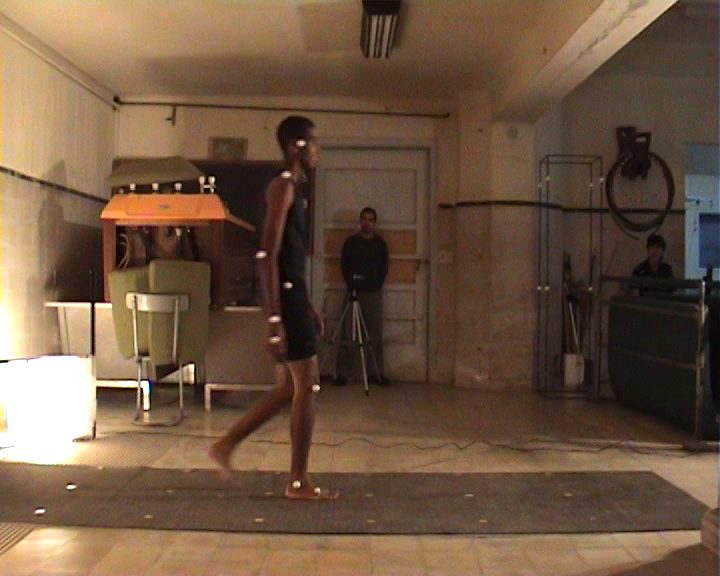
\includegraphics[scale=0.10]{imagenes/abel_original_video.png}\label{abelvideo}}\hspace{1 mm}
        {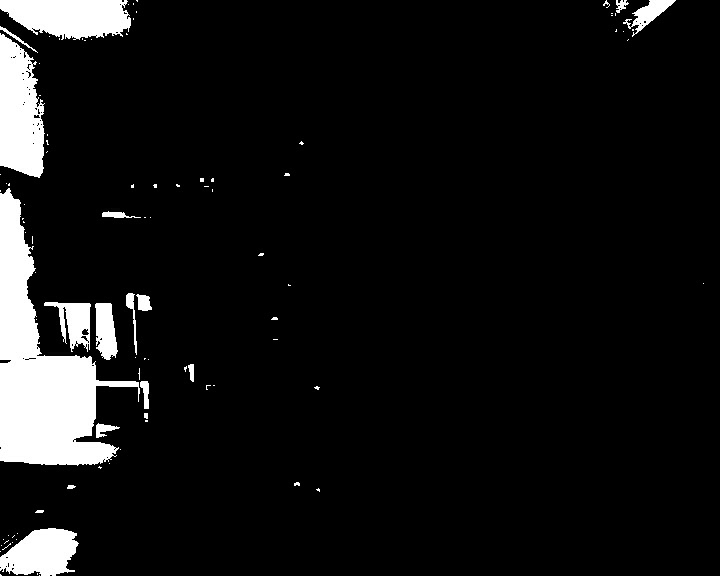
\includegraphics[scale=0.10]{imagenes/abel_original_filtro.png}\label{abelfiltro}}
        {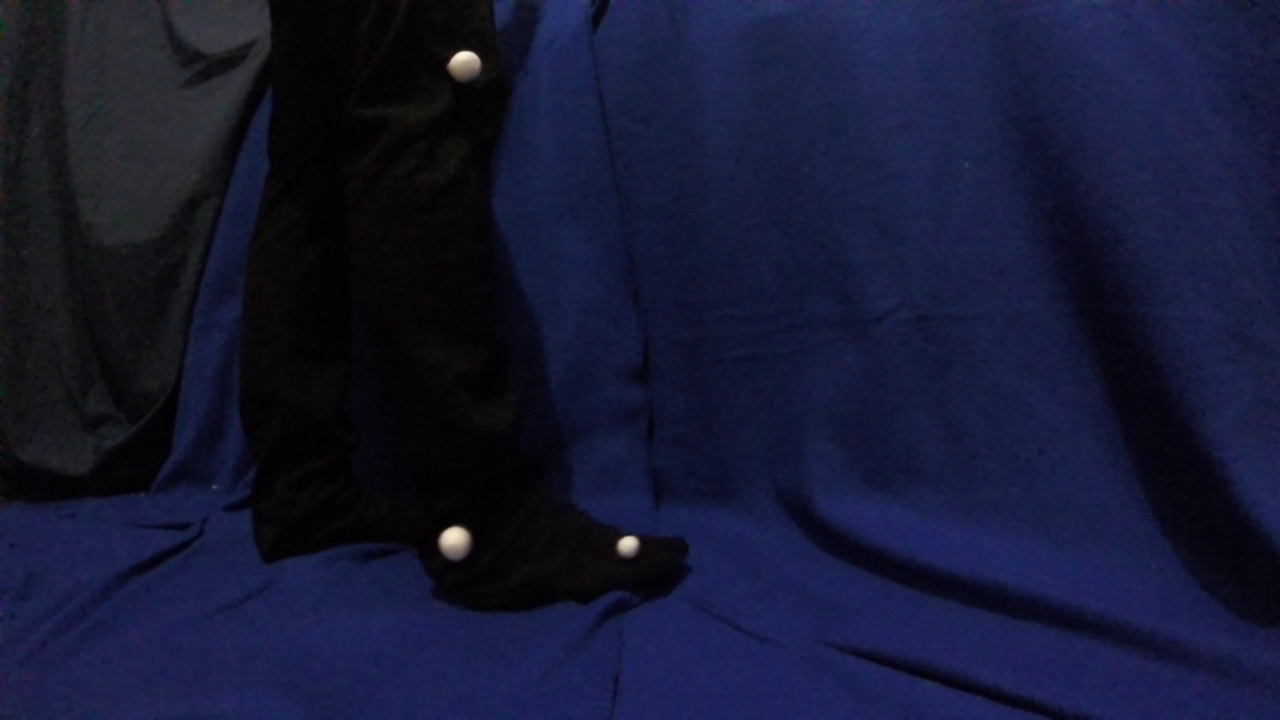
\includegraphics[scale=0.07]{imagenes/orig.png}\label{abelvideo2}}\hspace{1 mm}
       % {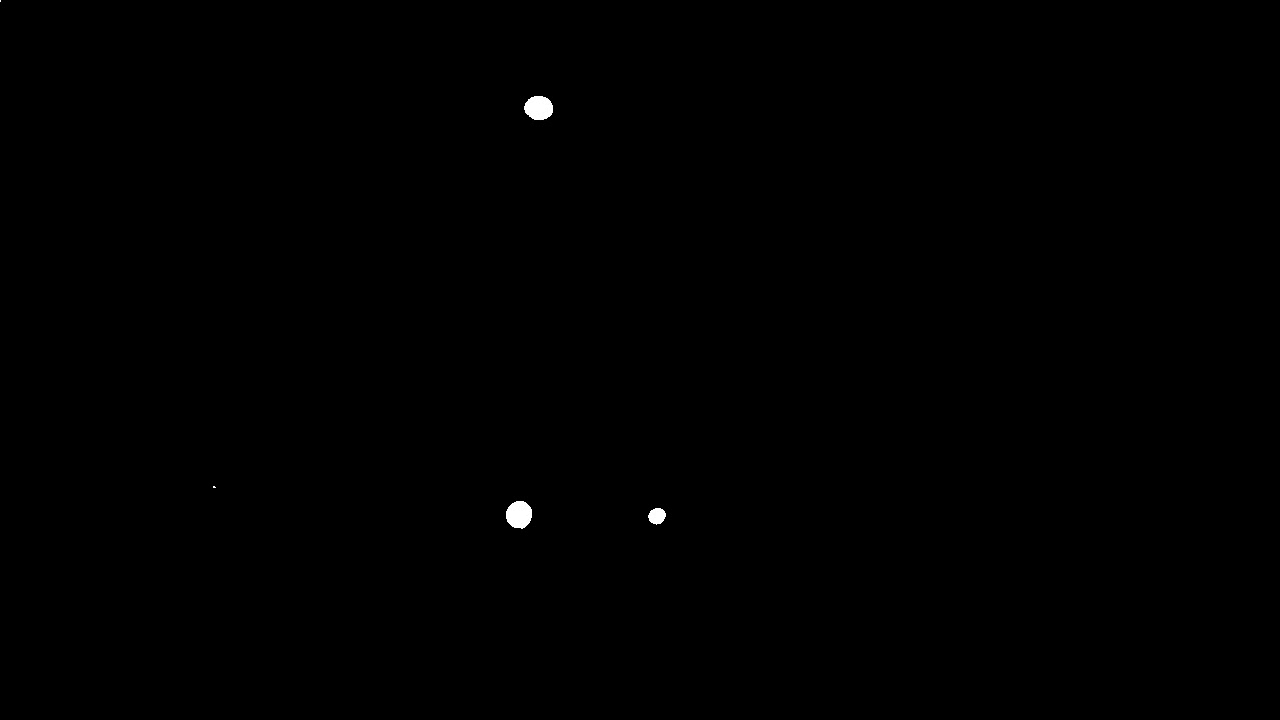
\includegraphics[scale=0.07]{imagenes/filtr.png}\label{abelfiltro2}}\hspace{1 mm}
        {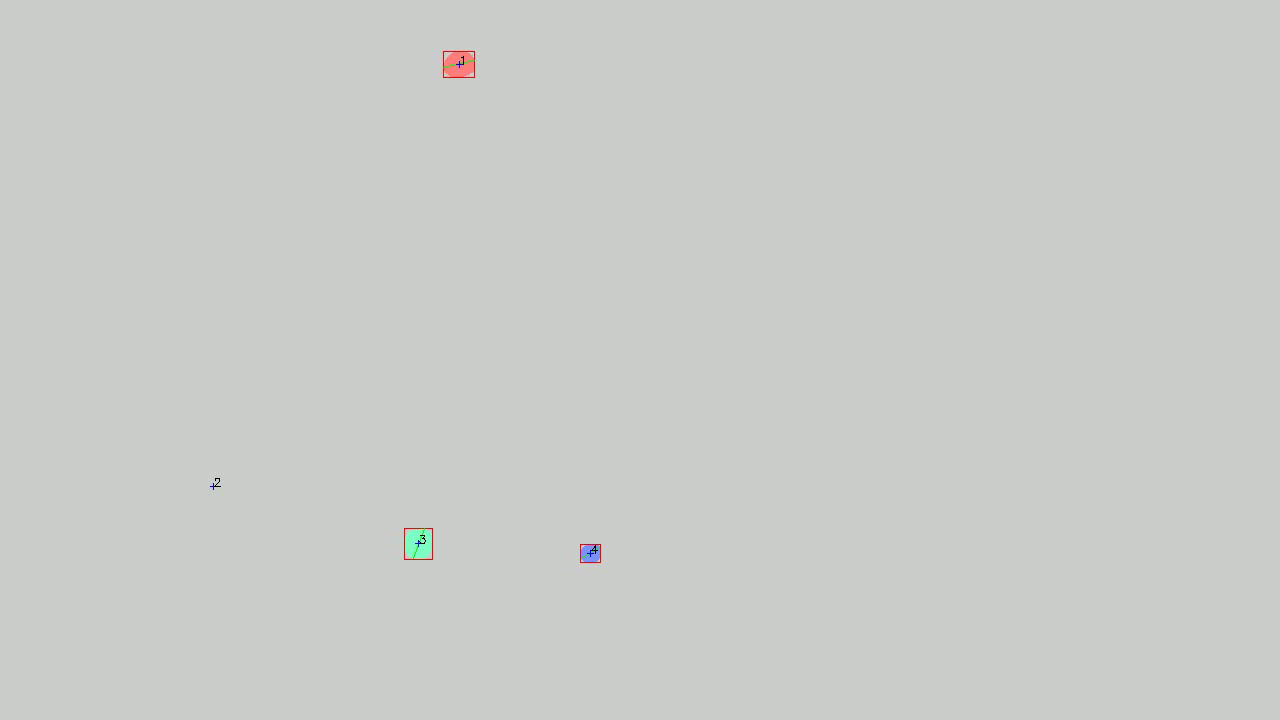
\includegraphics[scale=0.07]{imagenes/detect.png}
        \label{abeldetect}}
      \caption{%Entradas y salidas de cada etapa del bloque de deteción.
       %\textbf{(\ref{abelvideo})} 
       \textit{Izquierda}: imagen original de una secuencia fuera de las hipótesis de captura. 
       \textit{Centro izquierda}: resultado de la segmentación fuera de las hipótesis de captura.
       % \textbf{(\ref{abelvideo2})} 
       \textit{Centro derecha}: captura original de una secuencia real bajo las hipótesis de captura.
       % \textbf{(\ref{abelfiltro2})} Imagen filtrada con el umbral de Otsu. \textbf{(\ref{abeldetect})}
       \textit{Derecha}: marcadores detectados.}  
      \label{ejemploabelumbr2}
\end{figure}
\vspace{-0.6cm}